% Source for the figure of MPSCInbox (sec. 24.4): the stack of Treiber of
% the messages, after push(d) and after take(), which exchanges the top
% with nil and reverses the cells. Build: make figures (in ../build).
\documentclass[border=4pt]{standalone}
\usepackage[T1]{fontenc}
\usepackage{newpxtext,newpxmath}
\usepackage[varqu,varl,scaled=0.95]{zi4}
\usepackage{tikz}
% tikz-ads.tex: the TikZ styles shared by the figures of the memory of the
% manual, \input by each standalone figure: a cell of a vector (cell), the
% cell that an operation touches (touched), a free cell (free), a node of a
% linked structure (node), the labels of indices (index) and of variables
% (var), a pointer (ptr), and \cells and \indices to draw a row of cells.
\usetikzlibrary{arrows.meta,positioning,calc,fit,shapes.multipart}
\definecolor{adsTouched}{RGB}{214,196,236}
\definecolor{adsFree}{RGB}{236,236,236}
\tikzset{
  ads/.style={>={Stealth[length=2mm]},font=\small,
              every node/.append style={inner sep=0pt}},
  cell/.style={draw,minimum width=7mm,minimum height=7mm,
               font=\small\ttfamily,outer sep=0pt},
  touched/.style={cell,fill=adsTouched},
  free/.style={cell,fill=adsFree,text=black!45},
  node/.style={draw,rounded corners=1pt,minimum width=8mm,
               minimum height=6mm,font=\small\ttfamily},
  index/.style={font=\scriptsize\ttfamily,text=black!60},
  var/.style={font=\small\itshape},
  ptr/.style={->,thick}
}
% \cells{name}{x,y}{list}: a row of cells, the first at (x,y), named
% name-0, name-1, ...; each item is text/style, the style one of cell,
% touched and free (e.g., {a/cell,e/touched,/free})
\newcommand{\cells}[3]{%
  \foreach \v/\s [count=\i from 0] in {#3}
    \node[\s] (#1-\i) at ($(#2)+(\i*7mm,0)$) {\v};}
% \indices{name}{n}: the indices 0 .. n-1 under the cells of name
\newcommand{\indices}[2]{%
  \foreach \i in {0,...,\numexpr#2-1\relax}
    \node[index,below=1.2mm of #1-\i] {\i};}

\begin{document}
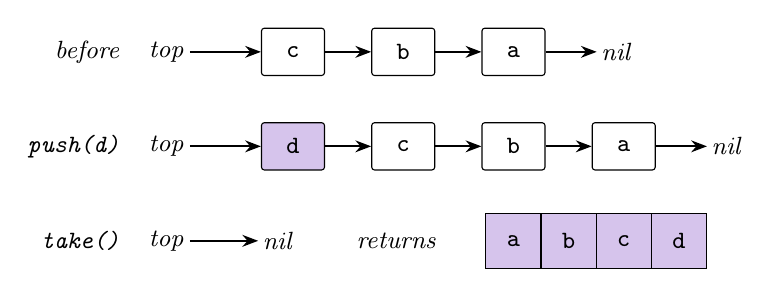
\begin{tikzpicture}[ads]
  \node[var,anchor=east] at (-6mm,0) {before};
  \node[var,inner sep=1.5pt] (top0) at (0,0) {$\mathit{top}$};
  \node[node] (c3) at (16mm,0) {c};
  \node[node] (c2) at (30mm,0) {b};
  \node[node] (c1) at (44mm,0) {a};
  \node[var,inner sep=1.5pt] (n0) at (57mm,0) {nil};
  \draw[ptr] (top0) -- (c3); \draw[ptr] (c3) -- (c2);
  \draw[ptr] (c2) -- (c1); \draw[ptr] (c1) -- (n0);
  \node[var,anchor=east] at (-6mm,-12mm) {\texttt{push(d)}};
  \node[var,inner sep=1.5pt] (top1) at (0,-12mm) {$\mathit{top}$};
  \node[node,fill=adsTouched] (d4) at (16mm,-12mm) {d};
  \node[node] (d3) at (30mm,-12mm) {c};
  \node[node] (d2) at (44mm,-12mm) {b};
  \node[node] (d1) at (58mm,-12mm) {a};
  \node[var,inner sep=1.5pt] (n1) at (71mm,-12mm) {nil};
  \draw[ptr] (top1) -- (d4); \draw[ptr] (d4) -- (d3);
  \draw[ptr] (d3) -- (d2); \draw[ptr] (d2) -- (d1); \draw[ptr] (d1) -- (n1);
  \node[var,anchor=east] at (-6mm,-24mm) {\texttt{take()}};
  \node[var,inner sep=1.5pt] (top2) at (0,-24mm) {$\mathit{top}$};
  \node[var,inner sep=1.5pt] (n2) at (14mm,-24mm) {nil};
  \draw[ptr] (top2) -- (n2);
  \node[var,anchor=west] at (24mm,-24mm) {returns};
  \cells{R}{44mm,-24mm}{a/touched,b/touched,c/touched,d/touched}
\end{tikzpicture}
\end{document}
